\documentclass[12pt,letterpaper]{article}\usepackage[]{graphicx}\usepackage[]{color}
%% maxwidth is the original width if it is less than linewidth
%% otherwise use linewidth (to make sure the graphics do not exceed the margin)
\makeatletter
\def\maxwidth{ %
  \ifdim\Gin@nat@width>\linewidth
    \linewidth
  \else
    \Gin@nat@width
  \fi
}
\makeatother

\definecolor{fgcolor}{rgb}{0.345, 0.345, 0.345}
\newcommand{\hlnum}[1]{\textcolor[rgb]{0.686,0.059,0.569}{#1}}%
\newcommand{\hlstr}[1]{\textcolor[rgb]{0.192,0.494,0.8}{#1}}%
\newcommand{\hlcom}[1]{\textcolor[rgb]{0.678,0.584,0.686}{\textit{#1}}}%
\newcommand{\hlopt}[1]{\textcolor[rgb]{0,0,0}{#1}}%
\newcommand{\hlstd}[1]{\textcolor[rgb]{0.345,0.345,0.345}{#1}}%
\newcommand{\hlkwa}[1]{\textcolor[rgb]{0.161,0.373,0.58}{\textbf{#1}}}%
\newcommand{\hlkwb}[1]{\textcolor[rgb]{0.69,0.353,0.396}{#1}}%
\newcommand{\hlkwc}[1]{\textcolor[rgb]{0.333,0.667,0.333}{#1}}%
\newcommand{\hlkwd}[1]{\textcolor[rgb]{0.737,0.353,0.396}{\textbf{#1}}}%

\usepackage{framed}
\makeatletter
\newenvironment{kframe}{%
 \def\at@end@of@kframe{}%
 \ifinner\ifhmode%
  \def\at@end@of@kframe{\end{minipage}}%
  \begin{minipage}{\columnwidth}%
 \fi\fi%
 \def\FrameCommand##1{\hskip\@totalleftmargin \hskip-\fboxsep
 \colorbox{shadecolor}{##1}\hskip-\fboxsep
     % There is no \\@totalrightmargin, so:
     \hskip-\linewidth \hskip-\@totalleftmargin \hskip\columnwidth}%
 \MakeFramed {\advance\hsize-\width
   \@totalleftmargin\z@ \linewidth\hsize
   \@setminipage}}%
 {\par\unskip\endMakeFramed%
 \at@end@of@kframe}
\makeatother

\definecolor{shadecolor}{rgb}{.97, .97, .97}
\definecolor{messagecolor}{rgb}{0, 0, 0}
\definecolor{warningcolor}{rgb}{1, 0, 1}
\definecolor{errorcolor}{rgb}{1, 0, 0}
\newenvironment{knitrout}{}{} % an empty environment to be redefined in TeX

\usepackage{alltt}
\usepackage[utf8]{inputenc}
\usepackage[margin=.7in]{geometry}
\usepackage{graphicx}
\usepackage{titling}
\usepackage{amsmath}
\usepackage{amsfonts}
\usepackage{amssymb}
\renewcommand{\theenumiv}{\arabic{enumiv}}
\setlength{\droptitle}{-5em}
\author{Maurice Diesendruck\vspace{-2ex}}
\title{StatMod2 - Hierarchical Models - Exercises 4\vspace{-1ex}}
\IfFileExists{upquote.sty}{\usepackage{upquote}}{}
\begin{document}
\maketitle

\section{School Averages and Sample Size}

Larger samples tend to "smooth" out extreme scores, so small samples are more 
likely to be extreme.\\

\begin{knitrout}
\definecolor{shadecolor}{rgb}{0.969, 0.969, 0.969}\color{fgcolor}\begin{kframe}
\begin{alltt}
\hlstd{data} \hlkwb{<-} \hlkwd{read.csv}\hlstd{(}\hlstr{"mathtest.csv"}\hlstd{)}
\hlkwd{attach}\hlstd{(data)}
\hlkwd{boxplot}\hlstd{(mathscore} \hlopt{~} \hlstd{school,} \hlkwc{xlab}\hlstd{=}\hlstr{"School"}\hlstd{,} \hlkwc{ylab}\hlstd{=}\hlstr{"Score"}\hlstd{)}
\end{alltt}
\end{kframe}
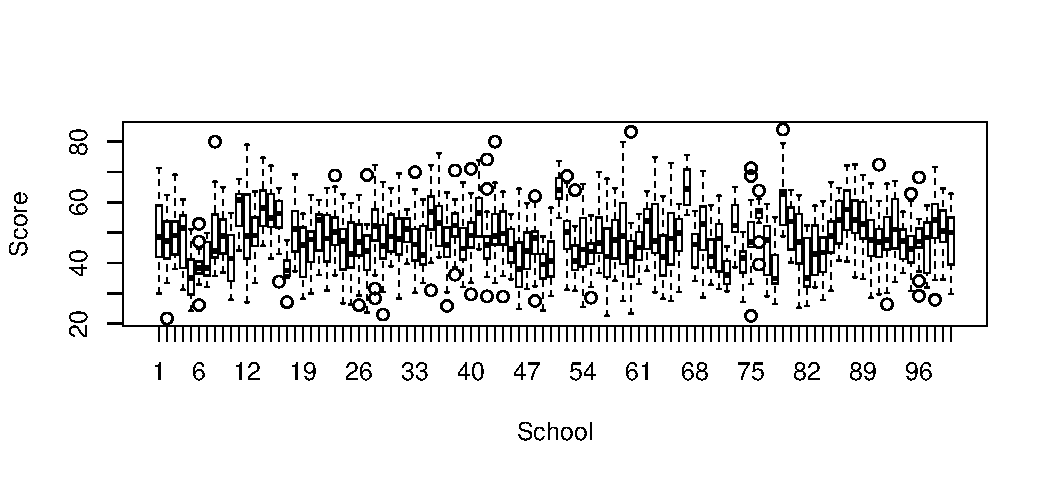
\includegraphics[width=\maxwidth]{figure/unnamed-chunk-1-1} 
\begin{kframe}\begin{alltt}
\hlstd{school.avgs} \hlkwb{<-} \hlkwd{aggregate}\hlstd{(data,} \hlkwd{list}\hlstd{(}\hlkwc{school}\hlstd{=school), mean)[,}\hlnum{3}\hlstd{]}
\hlstd{school.ssizes} \hlkwb{<-} \hlkwd{aggregate}\hlstd{(data,} \hlkwd{list}\hlstd{(}\hlkwc{school}\hlstd{=school), length)[,}\hlnum{3}\hlstd{]}
\hlkwd{plot}\hlstd{(}\hlkwd{cbind}\hlstd{(school.avgs, school.ssizes))}
\hlstd{fit} \hlkwb{<-} \hlkwd{lowess}\hlstd{(}\hlkwd{cbind}\hlstd{(school.avgs, school.ssizes))}
\hlkwd{lines}\hlstd{(fit)}
\end{alltt}
\end{kframe}
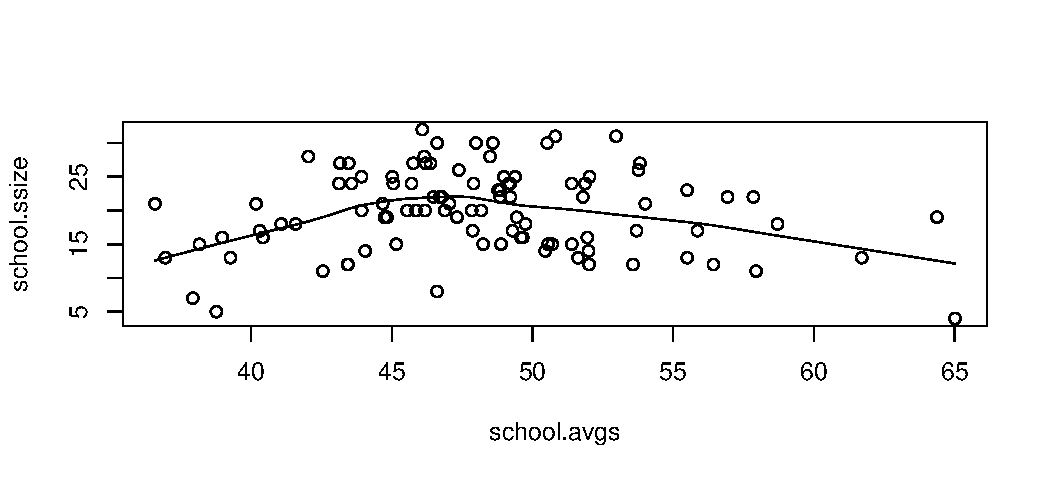
\includegraphics[width=\maxwidth]{figure/unnamed-chunk-1-2} 

\end{knitrout}

\section{Normal Hierarchical Model with Gibbs Sampling}

\subsection{Model}
For school $i=1,\cdots,p$; student $j=1,\cdots,n_i$; and $\sum n_i = n$; 
let $a=b=c=d=1$, and note that for this data, $p=100$ and $n=1993$:
\begin{align*}
  y_{ij} &\sim\ N(\theta_i,\sigma^2)\\
  \theta_i &\sim\ N(\mu,\tau^2)\\
  \mu &\sim\ Unif(40, 60)\\
  \sigma^2 &\sim\ InvGa(a,b)\\
  \tau^2 &\sim\ InvGa(c,d)\\
\end{align*}

Or alternatively,

\begin{align*}
  \bar{y_i} &\sim\ N(\theta_i,\frac{\sigma^2}{n_i})\\
  \theta_i &\sim\ N(\mu,\tau^2)\\
  \mu &\sim\ Unif(40, 60)\\
  \sigma^2 &\sim\ InvGa(a,b)\\
  \tau^2 &\sim\ InvGa(c,d)\\
\end{align*}
\begin{align*}
  N(\pmb{\bar{y}}|\pmb{\theta},\sigma^2 diag(1/n_i))
    N(\pmb{\theta}|\pmb{\mu}, \tau^2 I_p)
    Unif(\mu|40,60)
		Ga(\dfrac{1}{\sigma^2}|a, b) Ga(\dfrac{1}{\tau^2}|c, d)\\
\end{align*}


\subsection{Joint and Posterior Distributions}

Let $\pmb{\nu} = (\pmb{\theta}, \pmb{\mu}, \sigma^2, \tau^2)$; 
$\pmb{\theta}=\theta_1,\cdots,\theta_p$; 
$\pmb{\sigma_{*}^{2}} = \sigma^2 diag(1/n_i)$;
$\pmb{\bar{y}}$ be the $p$x$1$ vector
of mean math scores for all schools;
and note that $\pmb{\mu}$ is a $p$x$1$
vector with a single value, $\mu$.
\begin{align*}
  P(\pmb{\nu}|\pmb{y}) &\propto\ P(\pmb{y}|\pmb{\nu})P(\pmb{\nu})\\
  &= N(\pmb{\bar{y}}|\pmb{\theta},\pmb{\sigma_{*}^{2}})
    N(\pmb{\theta}|\pmb{\mu}, \tau^2 I_p)
    Unif(\mu|40,60)
  	Ga(\dfrac{1}{\sigma^2}|a, b) Ga(\dfrac{1}{\tau^2}|c, d)\\
  &= \Big( \frac{1}{\pmb{\sigma_{*}^{2}}} \Big) ^{p/2}
    exp \Big( -\frac{1}{2} \frac{(\pmb{\bar{y}}-\pmb{\theta})'
    (\pmb{\bar{y}}-\pmb{\theta})}{\pmb{\sigma_{*}^{2}}} \Big)\\
    &\hspace{10mm} \text{x } \Big( \dfrac{1}{\tau^2} \Big) ^{p/2}
			exp \Big( -\frac{1}{2} \Big( \dfrac{(\pmb{\theta}-\pmb{\mu})'
        (\pmb{\theta}-\pmb{\mu)}} {\tau^2} \Big)\Big)\\
		& \hspace{10mm} \text{x } \Big( \dfrac{1}{\sigma^2} \Big) 
			^{a-1} exp \Big( -b \Big( \dfrac{1}{\sigma^2} \Big) \Big)\\
		& \hspace{10mm} \text{x } \Big( \dfrac{1}{\tau^2} \Big) 
			^{c-1} exp \Big( -d \Big( \dfrac{1}{\tau^2} \Big) \Big)\\
%   &= \prod_{i=1}^p \Bigg[
%     \prod_{j\in \pmb{y_i}} N(y_{ij}|\theta_i,\sigma^2)
%     \Bigg]
%   	N(\pmb{\theta}|\pmb{\mu}, \tau^2 I_p)
%     Unif(\mu|40,60)
% 		Ga(\dfrac{1}{\sigma^2}|a, b) Ga(\dfrac{1}{\tau^2}|c, d)\\
% 	&\propto\ \prod_{i=1}^p \Bigg[
%     \Big( \dfrac{1}{\sigma^2} \Big) ^{n_i/2} 
% 		exp \Big( -\frac{1}{2} \Big( \dfrac{\sum_{j\in \pmb{y_i}}
%       (y_{ij}-\theta_i)^2}
% 			{\sigma^2} \Big) \Big) \Bigg]\\
% 		&\hspace{10mm} \text{x } \Big( \dfrac{1}{\tau^2} \Big) ^{p/2}
% 			exp \Big( -\frac{1}{2} \Big( \dfrac{(\pmb{\theta}-\pmb{\mu})'
%         (\pmb{\theta}-\pmb{\mu)}} {\tau^2} \Big)\Big)\\
% 		& \hspace{10mm} \text{x } \Big( \dfrac{1}{\sigma^2} \Big) 
% 			^{a-1} exp^{-b \Big( \dfrac{1}{\sigma^2} \Big)}\\
% 		& \hspace{10mm} \text{x } \Big( \dfrac{1}{\tau^2} \Big) 
% 			^{c-1} exp^{-d \Big( \dfrac{1}{\tau^2} \Big)}\\
\end{align*}

Conditional distributions are as follows:

\begin{align*}
P(\pmb{\theta}|\pmb{\bar{y}},\pmb{\mu}, \sigma^2, \tau^2) 
  &\propto\ exp \Big( -\frac{1}{2} \Big( \dfrac{(\pmb{\bar{y}}-\pmb{\theta})'
		(\pmb{\bar{y}}-\pmb{\theta})} {\pmb{\sigma_{*}^{2}}} + 
		\dfrac{(\pmb{\theta}-\pmb{\mu})'(\pmb{\theta}-\pmb{\mu})} {\tau^2}
		\Big) \Big)\\
	&= exp \Big( -\frac{1}{2} \Big( 
		\dfrac{\pmb{\bar{y}}'\pmb{\bar{y}}}{\pmb{\sigma_{*}^{2}}} -
    \dfrac{\pmb{\bar{y}}'\pmb{\theta}}{\pmb{\sigma_{*}^{2}}} -
    \dfrac{\pmb{\theta}'\pmb{\bar{y}}}{\pmb{\sigma_{*}^{2}}} +
    \dfrac{\pmb{\theta}'\pmb{\theta}}{\pmb{\sigma_{*}^{2}}} \Big) + \Big(
    \dfrac{\pmb{\theta}'\pmb{\theta}}{\tau^2} -
    \dfrac{\pmb{\theta}'\pmb{\mu}}{\tau^2} -
    \dfrac{\pmb{\mu}'\pmb{\theta}}{\tau^2} +
    \dfrac{\pmb{\mu}'\pmb{\mu}}{\sigma^2} \Big)
    \Big)\\
	&\sim\ N \Bigg( \Big( 
    \frac{I_n}{\pmb{\sigma_{*}^{2}}} +  \frac{I_n}{\tau^2} \Big) ^{-1}
		\Big( \frac{\pmb{\bar{y}}}{\pmb{\sigma_{*}^{2}}} - 
      \frac{\pmb{\mu}}{\tau^2} \Big) , 
		\Big( \frac{I_n}{\pmb{\sigma_{*}^{2}}} + \frac{I_n}{\tau^2} \Big) ^{-1}
		\Bigg)\\
\vspace{10mm}\\
P(\sigma^2|\pmb{y},\pmb{\theta},\tau^2) &\propto\
	\Big( \dfrac{1}{\sigma^2} \Big) ^{n/2}
	exp \Big( -\frac{1}{2} \Big( \dfrac{(\pmb{\bar{y}}-\pmb{\theta})'
			(\pmb{\bar{y}}-\pmb{\theta})} {\pmb{\sigma_{*}^{2}}} \Big) \Big)\\
	& \hspace{10mm} \text{x } \Big( \dfrac{1}{\sigma^2} \Big) 
			^{a-1} exp \Big( -b \Big( \dfrac{1}{\sigma^2} \Big) \Big)\\
	&= \Big( \dfrac{1}{\sigma^2} \Big) ^{n/2 + a -1}
		exp \Big( - \Big( \dfrac{(\pmb{\bar{y}}-\pmb{\theta})'
			(\pmb{\bar{y}}-\pmb{\theta})} {2 diag(1/n_i)} + b \Big)
			\Big( \frac{1}{\sigma^2} \Big) \Big)\\
	&\sim\ Ga \Big( n/2+a, \Big( \dfrac{(\pmb{\bar{y}}-\pmb{\theta})'
			(\pmb{\bar{y}}-\pmb{\theta})} {2 diag(1/n_i)} + b \Big) \Big)\\
\vspace{10mm}\\
P(\tau^2|\pmb{y},\pmb{\theta},\sigma^2) &\propto\
	\Big( \dfrac{1}{\tau^2} \Big) ^{p/2}
	exp \Big( -\frac{1}{2} \Big( \dfrac{(\pmb{\theta}-\pmb{\mu})'
    (\pmb{\theta}-\pmb{\mu})}{\tau^2}	\Big) \Big)\\
	& \hspace{10mm} \text{x } \Big( \dfrac{1}{\tau^2} \Big) 
			^{c-1} exp \Big( -d \Big( \dfrac{1}{\tau^2} \Big) \Big)\\
	&= \Big( \dfrac{1}{\tau^2} \Big) ^{p/2 + c -1}
		exp \Big( - \Big( \dfrac{(\pmb{\theta}-\pmb{\mu})'
      (\pmb{\theta}-\pmb{\mu})}{2} + d \Big)
			\Big( \frac{1}{\tau^2} \Big) \Big)\\
	&\sim\ Ga \Big( p/2+c, \Big( \dfrac{(\pmb{\theta}-\pmb{\mu})'
    (\pmb{\theta}-\pmb{\mu})}{2} + d \Big) \Big)\\
\vspace{10mm}
P(\pmb{\mu}|\pmb{y},\pmb{\theta}, \sigma^2, \tau^2) 
  &\propto\ exp \Big( -\frac{1}{2} \Big( 
  	\dfrac{(\pmb{\theta}-\pmb{\mu})'(\pmb{\theta}-\pmb{\mu})} {\tau^2}
		\Big) \Big)\\
  &\sim\ N(\pmb{\bar{\theta}}, \tau^2)
\end{align*}


\subsection{Gibbs Sampler}

\begin{knitrout}
\definecolor{shadecolor}{rgb}{0.969, 0.969, 0.969}\color{fgcolor}
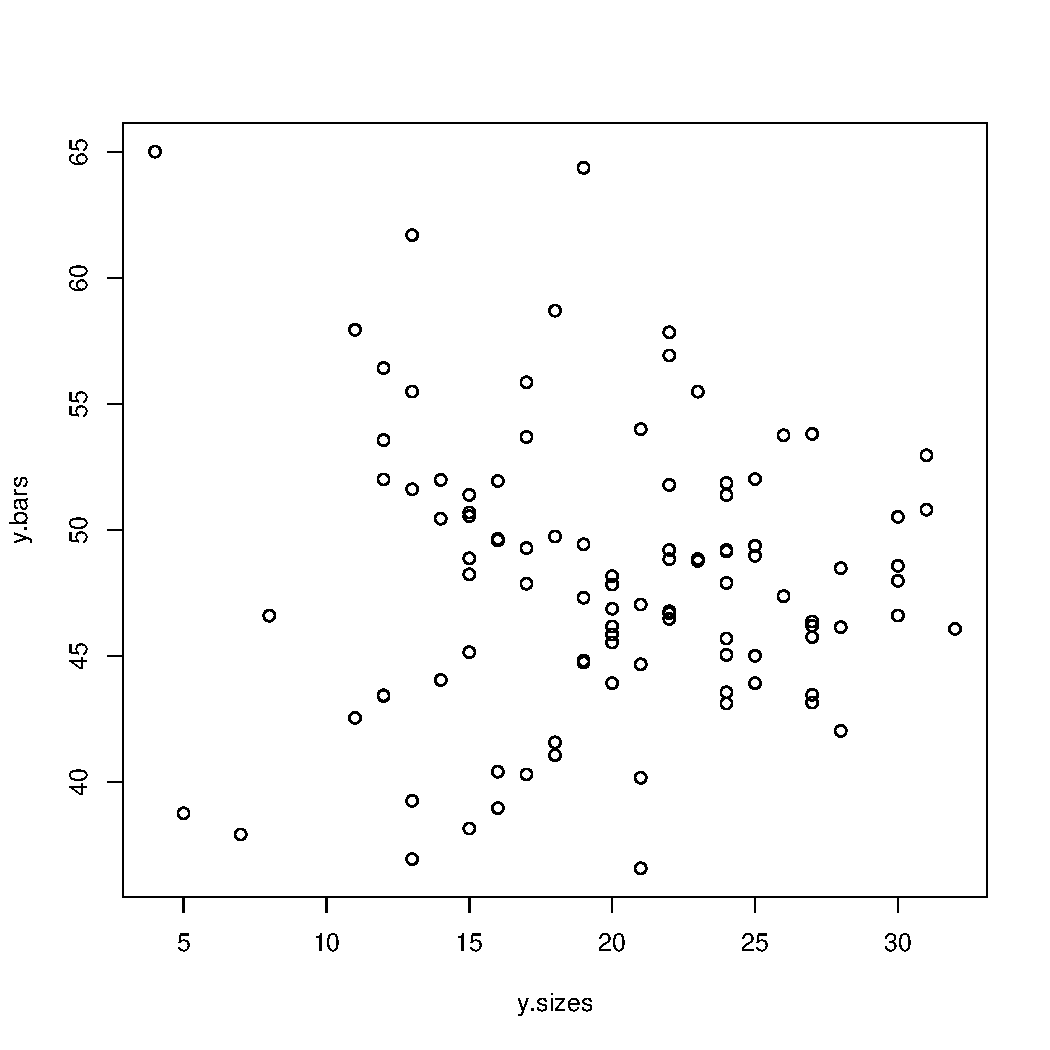
\includegraphics[width=\maxwidth]{figure/unnamed-chunk-2-1} 
\begin{kframe}

{\ttfamily\noindent\bfseries\color{errorcolor}{\#\# Error in eval(expr, envir, enclos): object 'ybars' not found}}\end{kframe}
\end{knitrout}

\subsection{Shrinkage}

In general, the smaller the sample size, the more extreme the sample mean, and the larger the shrinkage factor. 

\end{document}

